\documentclass{article}                         
\pagestyle{plain}

\usepackage{amsmath}     % Enhanced math environments (e.g., align).
\usepackage{amsfonts}    % Math fonts (e.g., \mathfrak{}).
\usepackage{amstext}     % Text inside math mode (e.g., \text{where}).
\usepackage{amssymb}     % Extra math symbols (e.g., \mathbb{R}).
\usepackage{array}       % Advanced table/array column definitions.
\usepackage{circledtext} % Puts text inside a circle (e.g., \circledtext{A}).
\usepackage{comment}     % Include/exclude blocks of text.
\usepackage{enumerate}   % Customize itemized/numbered lists.
\usepackage{geometry}    % Adjusts page margins and layout.
\usepackage{graphicx}    % Include images/graphics (\includegraphics).
\usepackage{latexsym}    % Access to basic LaTeX symbols.
\usepackage{multicol}    % Allows text columns on a page.
\usepackage{pgfplots}    % Create scientific plots from data (based on TikZ).
\usepackage{tabularx}    % Tables that stretch to page width.
\usepackage{tasks}       % Create multi-column lists.
\usepackage{textcomp}    % Provides many text symbols (e.g., \textcelsius).
\usepackage{tikz}        % Create vector graphics and diagrams.
\usepackage{xcolor}      % Define and use colors.
\usepackage{fancyhdr}
\usepackage{tcolorbox}
\geometry{a4paper, margin=1in}
\pagestyle{fancy}
\fancyhf{} % Clear all header and footer fields
\fancyhead[L]{Your Name} % Left header with name
\fancyhead[R]{October 21th 2025} % Right header with date
\renewcommand{\headrulewidth}{0.4pt} % Horizontal line below the header

\begin{document}

% Main title
\begin{center}
    \Large \textbf{Math 115E Activity 13} \\
    \vspace{0.2cm}
    \normalsize Chapter 5 Section 1-2 \\
    \normalsize Quadratics
\end{center}

\begin{tcolorbox}[
    width=\linewidth,
    colframe=black,         % Border color
    colback=white,          % Background color
    boxrule=0.5pt,          % Border thickness
    left=1mm, right=1.1mm,    % Horizontal padding
    top=1mm, bottom=1mm,    % Vertical padding
    arc=2mm                 % Corner radius
]
\textbf{Definition: Quadratic functions} 
\textit{are functions that can be written in the forms
\begin{itemize}
    \item \textbf{Standard Form}: $f(x)=ax^2+bx+c$ \\
        where $a,b,c$ are real numbers and $a \neq 0$
    \item \textbf{Vertex Form}: $f(x)=a(x-h)^2+k$ \\
        where $a,b,k$ are real numbers with the point $(h,k)$ being the vertex
\end{itemize}
}
\end{tcolorbox}
\noindent
\textbf{Section 1: Identifying Quadratic functions from a graph}

\begin{minipage}[c]{0.45\textwidth}
    \vspace{-4cm}
    \begin{enumerate}
        
        \item Determine the y-intercept,
        x-intercepts, vertex and max/min of the function
        \vspace{5cm}

        \item Determine the y-intercept,
        x-intercepts, vertex and max/min of the function
        \vspace{5cm}

        \item Determine the y-intercept,
        x-intercepts, vertex and max/min of the function   


    \end{enumerate}
\end{minipage}%
\hfill
\begin{minipage}[c]{0.50\textwidth} % Minipage for the TikZ graph (increased width slightly for labels)
    \centering % Center the TikZ picture within its minipage
    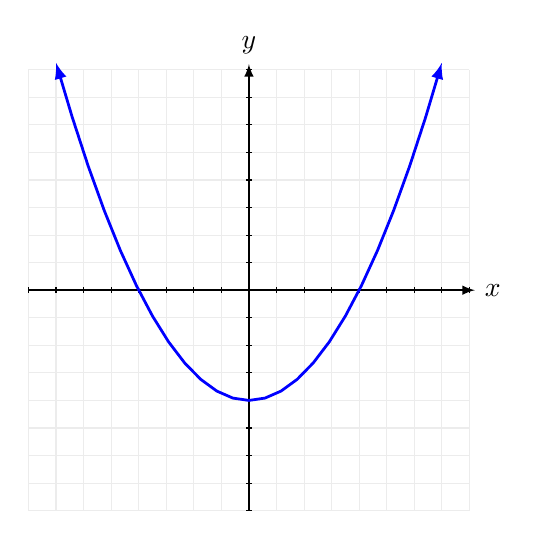
\begin{tikzpicture}[scale=0.35]
        \draw[gray!15,step=1cm] (-8,-8) grid (8,8);
        \draw[line width=0.2mm, -latex] (-8,0) -- (8.2,0) node[right] {$x$};
        % The \foreach loop for x-axis numbers has been modified
        \foreach \x in {-8,...,8} \draw (\x,.1)--(\x,-.1);
        \draw[line width=0.2mm,  -latex] (0,-8) -- (0,8.2) node[above] {$y$};
        % The \foreach loop for y-axis numbers has been modified
        \foreach \y in {-8,...,8} \draw (.1,\y)--(-.1,\y);
        % Blue line with adjusted label 'A'
        \draw[blue,line width=1pt, latex-latex] plot[domain= -7:7] (\x,{0.25*\x*\x-4}) node[font=\tiny] {};    
    \end{tikzpicture}
    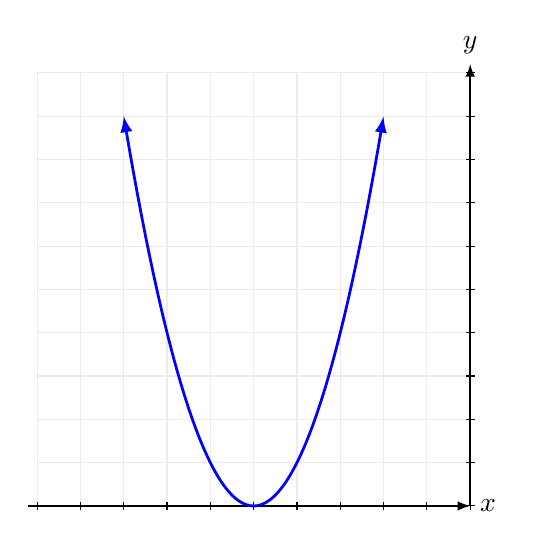
\begin{tikzpicture}[scale=0.55]
        \draw[gray!15,step=1cm] (-10,10) grid (0,0);
        \draw[line width=0.2mm, -latex] (-10.2,0) -- (0,0) node[right] {$x$};
        % The \foreach loop for x-axis numbers has been modified
        \foreach \x in {-10,...,0} \draw (\x,.1)--(\x,-.1);
        \draw[line width=0.2mm,  -latex] (0,0) -- (0,10.2) node[above] {$y$};
        % The \foreach loop for y-axis numbers has been modified    
        \foreach \y in {0,...,10} \draw (.1,\y)--(-.1,\y);
        % Blue line with adjusted label 'B'
        \draw[blue,line width=1pt, latex-latex] plot[smooth, samples=100, domain=-8:-2] (\x,{(\x+5)*(\x+5)}) node[font=\tiny] {};

    \end{tikzpicture}
    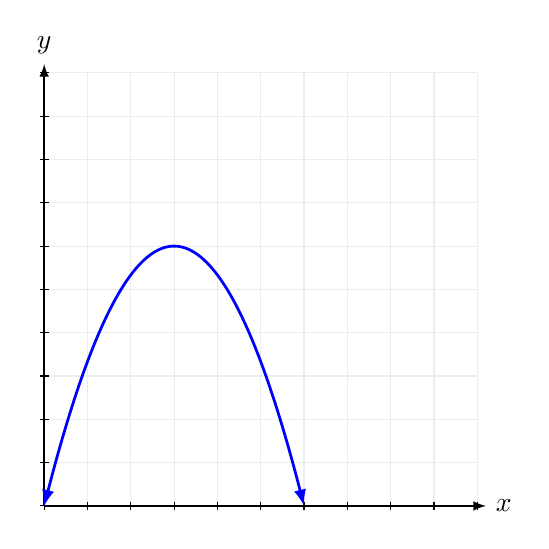
\begin{tikzpicture}[scale=0.55]
        \draw[gray!15,step=1cm] (0,0) grid (10,10);
        \draw[line width=0.2mm, -latex] (0,0) -- (10.2,0) node[right] {$x$};
        % The \foreach loop for x-axis numbers has been modified
        \foreach \x in {0,...,10} \draw (\x,.1)--(\x,-.1);
        \draw[line width=0.2mm,  -latex] (0,0) -- (0,10.2) node[above] {$y$};
        % The \foreach loop for y-axis numbers has been modified
        \foreach \y in {0,...,10} \draw (.1,\y)--(-.1,\y);  
        % Blue line with adjusted label 'B'
        \draw[blue,line width=1pt, latex-latex] plot[smooth, samples=100, domain= 0:6] (\x,{-(2/3)*(\x)*(\x-6)}) node[font=\tiny] {};

    \end{tikzpicture}
\end{minipage}

\vspace{1cm}
\noindent

\noindent
\textbf{Section 2: Factoring a quadratic expression}

\begin{tcolorbox}[
    width=\linewidth,
    colframe=black,         % Border color
    colback=white,          % Background color
    boxrule=0.5pt,          % Border thickness
    left=1mm, right=1.1mm,    % Horizontal padding
    top=1mm, bottom=1mm,    % Vertical padding
    arc=2mm                 % Corner radius
]
\textbf{Helpful Tips: } 
\textit{When factoring, the form $x^2 + bx + c$ can be factored as $(x+m)(x+n)$\\
\hspace*{2.5cm} with real numbers $m$ and $n$ such that: they both multiply to $c$ and yet both add to $b$}
\end{tcolorbox}


\begin{minipage}[t]{0.45\textwidth}
    \begin{enumerate}
        \item Factor $x^2 + x - 6$
        \\\\\\\\\\\\\\
        \item Factor $x^2 - x - 6$
        \\\\\\\\\\\\\\
        \item Factor $x^2 - 9x + 20$
        \\\\\\\\\\\\\\
        \item Factor $x^2 + 7x + 6$
        \\\\\\\\\\\\\\
        \item Factor $x^2 - 2x - 80$
        \\\\\\\\\\\\\\
        \item Factor $x^2 - 13x + 42$
        
        
    \end{enumerate}
\end{minipage}%
\hfill
\begin{minipage}[t]{0.45\textwidth}
    \begin{enumerate}
        \setcounter{enumi}{4} % continues numbering
        \item Factor $x^2 - 4$
        \\\\\\\\\\\\\\
        \item Factor $x^2 + 2x - 120$
        \\\\\\\\\\\\\\
        \item Factor $x^2 + 22x + 120$
        \\\\\\\\\\\\\\
        \item Factor $x^2 + 18x + 32$
        \\\\\\\\\\\\\\
        \item Factor $x^2 + 26x + 160$
        \\\\\\\\\\\\\\
        \item Factor $x^2 + 33x + 200$
        

    \end{enumerate}
\end{minipage}

\end{document}